\section{Joint asymptotics for reflected log-gamma moments}
\label{cont26:joint:sec:main}

Let
\[
 f(x)=\log\Gamma(x),\qquad B(x)=f(1-x),\qquad
 M_{n,m}=\int_0^1 f(x)^n B(x)^m\,dx.
\]
These mixed integrals are classical; they occur as $T_{n+m,n}$ in
\cite[Section~5]{ACEMKM}.  The fixed-$m$ expansions in the
repository do not give relative estimates when both exponents grow.
This section treats two parts of that unresolved regime.  First, a
global uniqueness theorem gives a full saddle expansion whenever
$m/n$ remains in a compact subset of $(0,\infty)$.  Second, an entirely
analytic transition theorem determines exactly how the leading
fixed-$m$ approximation fails near $n/(m+1)=\log m+O(1)$.
The first result uses a short, reproducible rational certificate for a
special-function inequality.  The transition theorem does not depend
on that certificate.

All exponents in this section may be positive real numbers; the
factorial $n!$ is then written $\Gamma(n+1)$.  The familiar inequalities
$0<f(x)\le-\log x$ on $(0,1)$ follow from $\psi(1)=-\gamma<0$,
$\psi'(x)>0$, and log-convexity of $\Gamma$ between $1$ and $2$.
The Taylor series and polygamma formulas used below are classical
\cite{DLMFTaylor,DLMFPolygamma}.

\subsection{A strict monotonicity theorem and one saddle for every ratio}

Define positive functions
\begin{equation}\label{cont26:joint:eq:hQ}
 h(x)=\frac{-\psi(x)}{\log\Gamma(x)},\qquad
 Q(x)=\frac{h(x)}{h(1-x)},\qquad 0<x<1.
\end{equation}
Direct differentiation gives
\begin{align}\label{cont26:joint:eq:D}
 D(x):=\frac{d}{dx}\log Q(x)
 ={}&\frac{-\psi(x)}{f(x)}+
     \frac{-\psi(1-x)}{f(1-x)}\notag\\
 &-\frac{\psi'(x)}{-\psi(x)}-
     \frac{\psi'(1-x)}{-\psi(1-x)}.
\end{align}

\begin{theorem}[Strict reflected elasticity inequality]
\label{cont26:joint:thm:Q}
For every $0<x<1$, $D(x)>0$.  Consequently $Q$ is a strictly increasing
real-analytic bijection from $(0,1)$ onto $(0,\infty)$, and
$Q(1-x)=Q(x)^{-1}$.  In particular,
\begin{equation}\label{cont26:joint:eq:product}
 \log\Gamma(x)\log\Gamma(1-x)
 \le \frac{\log^2\pi}{4},
\end{equation}
with equality exactly at $x=1/2$.
\end{theorem}

\begin{proof}
The identity $D(1-x)=D(x)$ reduces the problem to $0<x\le1/2$.
We first give an analytic proof on $0<x\le1/16$, and then describe the
finite rational certificate for $1/16\le x\le1/2$.

Write $L=-\log x$, $p=-\psi(x)$, $s=-\psi(1-x)$, and
$b=B(x)/x$.  The positive series
\[
 B(x)=\gamma x+\sum_{k\ge2}\frac{\zeta(k)}k x^k
\]
implies $s/b\ge1$ and $s\ge\gamma>1/2$.
Concavity of $\psi$ gives
$\psi(1+x)\le-\gamma+\zeta(2)x<0$ on this interval.
Thus $xp=1-x\psi(1+x)\ge1$, and $f(x)\le L$ gives
$xp/f(x)\ge1/L$.  The polygamma series yield
\[
 x^2\psi'(x)=1+x^2\psi'(1+x)\le1+2x^2,
 \qquad \psi'(1-x)\le\frac{\zeta(2)}{(1-x)^2}
 <\frac2{(1-x)^2}.
\]
Inserting these inequalities into \eqref{cont26:joint:eq:D} gives
\begin{equation}\label{cont26:joint:eq:endpoint-D}
 xD(x)\ge\frac1L-2x^2-\frac{4x}{(1-x)^2}>0.
\end{equation}
For the last inequality, $xL$ and $x^2L$ increase on $(0,1/16]$,
and $\log16<3$.  Therefore
\[
 L\left(2x^2+\frac{4x}{(1-x)^2}\right)
 \le\log16\left(\frac1{128}+\frac{64}{225}\right)
 <\frac{25251}{28800}<1.
\]

For the remaining compact interval, set
\[
 p_1=-\psi(x),\quad p_2=-\psi(1-x),\quad
 v_1=\psi'(x),\quad v_2=\psi'(1-x),\quad f_1=f(x),\quad f_2=B(x).
\]
The functions $f_1,p_1,v_1$ decrease, and $f_2,p_2,v_2$ increase.
If $a\le x\le b$, interval enclosures at the two endpoints therefore give
the rigorous rational lower bound
\begin{equation}\label{cont26:joint:eq:certificate-lower}
 D(x)\ge
 \frac{\underline p_1(b)}{\overline f_1(a)}
 +\frac{\underline p_2(a)}{\overline f_2(b)}
 -\frac{\overline v_1(a)}{\underline p_1(b)}
 -\frac{\overline v_2(b)}{\underline p_2(a)}.
\end{equation}
All denominators are positive.  Use the 112 intervals
$[j/256,(j+1)/256]$, $16\le j<128$, and the explicit enclosures in
Subsection~\ref{cont26:joint:subsec:certificate}.  Exact rational evaluation of
\eqref{cont26:joint:eq:certificate-lower}, reproduced by
\texttt{certify\_gamma\_saddle.py}, proves on every interval that
\begin{equation}\label{cont26:joint:eq:certificate-margin}
 D(x)\ge \frac{1693471917}{10^9}>0.
\end{equation}
The complete list of rational lower bounds is stored in
\texttt{gamma\_saddle\_certificate.json}.  Neither special-function
floating-point evaluations nor numerical differentiation enter these
checks.  This finite certificate completes the inequality on $(0,1)$.

Finally, $f(x)\sim-\log x$, $-\psi(x)\sim1/x$, and
$f(1-x)\sim\gamma x$ as $x\downarrow0$, so
$Q(x)\sim1/\log(1/x)\to0$.  Reflection gives the limit $+\infty$ at
one.  The derivative of the logarithm of the product in
\eqref{cont26:joint:eq:product} is $h(1-x)(1-Q(x))$.
Its unique zero is $x=1/2$, with positive derivative sign before that
point and negative sign afterward.  Since $\Gamma(1/2)=\sqrt\pi$,
the sharp bound and equality case follow.
\end{proof}

\begin{theorem}[Uniform joint saddle expansion]
\label{cont26:joint:thm:laplace}
Let $\lambda=m/n$ remain in a fixed compact subset $K\subset(0,\infty)$
as $n\to\infty$.  Let $x_\lambda$ be the unique solution of
\begin{equation}\label{cont26:joint:eq:saddle}
 Q(x_\lambda)=\lambda,
\end{equation}
and define
\[
 \Phi_\lambda(x)=\log f(x)+\lambda\log f(1-x),\qquad
 \kappa_\lambda=-\Phi_\lambda''(x_\lambda)>0.
\]
Then, uniformly for $\lambda\in K$,
\begin{align}\label{cont26:joint:eq:laplace}
 M_{n,m}={}&f(x_\lambda)^n f(1-x_\lambda)^m
 \sqrt{\frac{2\pi}{n\kappa_\lambda}}
 \left(1+\frac{C_1(\lambda)}n+O_K(n^{-2})\right),\\
 C_1(\lambda)={}&
 \frac{\Phi_\lambda^{(4)}(x_\lambda)}{8\kappa_\lambda^2}
 +\frac{5\Phi_\lambda^{(3)}(x_\lambda)^2}{24\kappa_\lambda^3}.
 \label{cont26:joint:eq:C1}
\end{align}
There is a full uniform expansion in integer powers of $1/n$.
Moreover $x_\lambda$ increases analytically from zero to one as
$\lambda$ increases from zero to infinity, and
$x_{1/\lambda}=1-x_\lambda$.
\end{theorem}

\begin{proof}
By \eqref{cont26:joint:eq:hQ},
\[
 \Phi_\lambda'(x)=h(1-x)(\lambda-Q(x)).
\]
Theorem~\ref{cont26:joint:thm:Q} proves that this is positive before
$x_\lambda$ and negative after it.  It also proves nondegeneracy:
\begin{equation}\label{cont26:joint:eq:curvature}
 \kappa_\lambda=h(1-x_\lambda)Q'(x_\lambda)>0.
\end{equation}
The analytic implicit-function theorem proves the assertions about
$x_\lambda$; reflection gives the last identity.

Compactness of $K$ keeps $x_\lambda$ a fixed distance from both
endpoints, and bounds $\kappa_\lambda$ away from zero.  All required
derivatives of the phase are then uniformly bounded in one fixed
neighborhood of the moving saddle.  The phase tends to $-\infty$
at either endpoint, uniformly for $\lambda\in K$: near zero it is
$\log\log(1/x)+\lambda\log x+O_K(1)$, and near one the analogous
formula follows by reflection.  Strict unimodality and compactness
give a uniform positive gap between the maximum and the phase
outside a fixed neighborhood of the saddle.  Thus the integral over
that complement is exponentially smaller than the saddle term.

In the neighborhood, put $u=\sqrt{n\kappa_\lambda}(x-x_\lambda)$
and Taylor-expand the analytic phase.  Gaussian domination justifies
termwise integration to every fixed order.  Odd powers integrate to
zero; the quartic term and the square of the cubic term give
\eqref{cont26:joint:eq:C1}.  To make the error assertion explicit, expand
through enough even orders on $|u|\le n^{1/10}$, use the uniform
Taylor remainder there, and bound its complement by
$O(e^{-c n^{1/5}})$.  This proves the stated relative error and full
uniform expansion without an unproved competing-saddle assumption.
\end{proof}

For reproducibility, the coefficient $C_j$ at arbitrary order can be
written as a finite sum.  All derivatives below are evaluated at
$x_\lambda$.  For nonnegative integers $r_3,\ldots,r_{2j+2}$ with
$\sum_{k=3}^{2j+2}(k-2)r_k=2j$, put
$R=\sum_{k=3}^{2j+2}k r_k$.  Then
\begin{equation}\label{cont26:joint:eq:allorders}
 C_j(\lambda)=
 \sum_{\sum(k-2)r_k=2j}
 \frac{(R-1)!!}{\kappa_\lambda^{R/2}}
 \prod_{k=3}^{2j+2}
 \frac1{r_k!}\left(\frac{\Phi_\lambda^{(k)}}{k!}\right)^{r_k},
\end{equation}
with $C_0=1$ and $(-1)!!=1$.  The constraint makes $R$ even.
This is simply coefficient extraction after expanding the exponential
of the terms of degree at least three in the local phase.

\begin{corollary}[Equal exponents]
\label{cont26:joint:cor:diagonal}
Set
\[
 a=\frac{\log\pi}{2},\qquad p=\gamma+2\log2,\qquad
 \kappa=\frac{2}{a^2}\left(p^2-\frac{\pi^2a}{2}\right).
\]
Then $\kappa>0$ and
\begin{equation}\label{cont26:joint:eq:diagonal}
 M_{n,n}=a^{2n}\sqrt{\frac{2\pi}{n\kappa}}
 \left(1+\frac{c_*}{n}+O(n^{-2})\right),
 \qquad c_*=-0.4398093541949199\ldots.
\end{equation}
The constant is exactly $c_*=\Phi_1^{(4)}(1/2)/(8\kappa^2)$, where
\begin{equation}\label{cont26:joint:eq:diagonal-fourth}
 \Phi_1^{(4)}(1/2)=2\left[
 \frac{\pi^4}{a}
 -\frac{56p\zeta(3)+3\pi^4/4}{a^2}
 +\frac{6p^2\pi^2}{a^3}
 -\frac{6p^4}{a^4}\right].
\end{equation}
Numerically $\kappa=6.2933987786891021\ldots$ and
$\sqrt{2\pi/\kappa}=0.9991882272949156\ldots$.
\end{corollary}
\begin{proof}
Here $x_1=1/2$ and all odd phase derivatives vanish.  Use
$\psi(1/2)=-p$, $\psi'(1/2)=\pi^2/2$,
$\psi''(1/2)=-14\zeta(3)$, and $\psi^{(3)}(1/2)=\pi^4$ in
Theorem~\ref{cont26:joint:thm:laplace}.  Differentiating $\log f$ four
times gives \eqref{cont26:joint:eq:diagonal-fourth}.
\end{proof}

\subsection{The compact interval certificate in full}
\label{cont26:joint:subsec:certificate}

This subsection specifies the arithmetic proof object independently
of any special-function library.  Every input is rational, and each
infinite tail has an explicit rational bound.

For $1\le z\le2$, put $y=(z-1)/(z+1)$ and use
\begin{equation}\label{cont26:joint:eq:log-bound}
 0\le\log z-2\sum_{r=0}^{31}\frac{y^{2r+1}}{2r+1}
 \le\frac{2y^{65}}{65(1-y^2)}.
\end{equation}
For any positive rational input, multiplication by an integral power
of two reduces its logarithm to this interval; $\log2$ is enclosed
by the same formula.  This controls all logarithms in the proof.

Euler's constant is enclosed with $N=32$ by
\begin{equation}\label{cont26:joint:eq:gamma-bound}
 H_N-\log N-\frac1{2N}<\gamma<
 H_N-\log N-\frac1{2N}+\frac1{12N^2}.
\end{equation}
For a short elementary verification, set
$e_N=H_N-\log N-1/(2N)$ and $z=1/(2N+1)$.
Expansion of $\log((1+z)/(1-z))$ gives
\[
 e_{N+1}-e_N=
 4\sum_{r\ge1}\frac{r}{2r+1}z^{2r+1}>0.
\]
The sequence $u_N=e_N+1/(12N^2)$ decreases, since
\[
 u_N-u_{N+1}=
 \sum_{r\ge1}\frac{8r(r-1)}{3(2r+1)}z^{2r+1}>0.
\]
Both sequences tend to $\gamma$, proving \eqref{cont26:joint:eq:gamma-bound}.
The certificate also verifies $1/2<\gamma<2/3$.
For each integer $k\ge2$, the elementary integral test gives
\begin{equation}\label{cont26:joint:eq:zeta-bound}
 \sum_{r=1}^{32}\frac1{r^k}+\frac{33^{1-k}}{k-1}
 \le\zeta(k)\le
 \sum_{r=1}^{32}\frac1{r^k}+\frac{32^{1-k}}{k-1}.
\end{equation}
In particular $1<\zeta(k)<2$.

For each grid endpoint $x\in[1/16,1/2]$, use the degree-40 series
\begin{align*}
 f_1(x)&=-\log x-\gamma x+
       \sum_{k=2}^{40}\frac{(-1)^k\zeta(k)}k x^k+\varepsilon_f,\\
 f_2(x)&=\gamma x+
       \sum_{k=2}^{40}\frac{\zeta(k)}k x^k+\varepsilon_B,\\
 p_1(x)&=x^{-1}+\gamma+
       \sum_{k=2}^{40}(-1)^{k+1}\zeta(k)x^{k-1}+\varepsilon_p,\\
 p_2(x)&=\gamma+
       \sum_{k=2}^{40}\zeta(k)x^{k-1}+\varepsilon_s,\\
 v_1(x)&=x^{-2}+
       \sum_{k=2}^{40}(-1)^k(k-1)\zeta(k)x^{k-2}+\varepsilon_v,\\
 v_2(x)&=\sum_{k=2}^{40}(k-1)\zeta(k)x^{k-2}+\varepsilon_u.
\end{align*}
With
\[
 E_f=\frac{2x^{41}}{41(1-x)},\qquad
 E_p=\frac{2x^{40}}{1-x},\qquad
 E_v=2x^{39}\left(\frac{40}{1-x}+\frac{x}{(1-x)^2}\right),
\]
one has $|\varepsilon_f|\le E_f$,
$|\varepsilon_p|\le E_p$, $|\varepsilon_v|\le E_v$,
and $0\le\varepsilon_B\le E_f$,
$0\le\varepsilon_s\le E_p$, $0\le\varepsilon_u\le E_v$.
These follow by bounding each omitted $\zeta(k)$ by two and summing
a geometric series or its derivative.

Substitute the rational intervals from
\eqref{cont26:joint:eq:log-bound}--\eqref{cont26:joint:eq:zeta-bound} with the correct
sign into these six formulas.  Evaluate
\eqref{cont26:joint:eq:certificate-lower} on the 112 adjacent intervals.
The smallest lower bound, rounded downward to denominator $10^9$,
is the number in \eqref{cont26:joint:eq:certificate-margin}; it occurs on
$[127/256,1/2]$.  This completely specifies the finite verification.
The following command replays all the fraction operations and compares
the stored proof object:
\begin{quote}\ttfamily
 python certify\_gamma\_saddle.py --check
\end{quote}
The script uses only the Python standard library and has no numerical
special-function dependency.  The role of the computation is the
finite family of strict rational inequalities, whose analytic coverage
has already been proved.  Replacing it by a short conceptual proof of
\eqref{cont26:joint:eq:D} is a useful further question.

\subsection{The small-ratio saddle has an exponential transseries}

The saddle approaches the endpoint on an exponential scale when
$\lambda\downarrow0$.  Define
\begin{equation}\label{cont26:joint:eq:cde}
 c=\frac{\zeta(2)}{2\gamma},\qquad d=c-\gamma,\qquad
 e=\gamma^2+\frac{\zeta(3)}{3\gamma}
                   -\frac{\zeta(2)^2}{8\gamma^2}.
\end{equation}
Here $d>0$: $\gamma<2/3$ and $\zeta(2)>1$ suffice.

\begin{proposition}[Endpoint location of the moving saddle]
\label{cont26:joint:prop:saddle-small}
As $\lambda\downarrow0$,
\begin{equation}\label{cont26:joint:eq:saddle-small}
 x_\lambda=e^{-1/\lambda}
 \left[1+\left(\frac d\lambda-\gamma\right)e^{-1/\lambda}
 +O\left(\lambda^{-2}e^{-2/\lambda}\right)\right].
\end{equation}
The corresponding expansion near $\lambda=\infty$ follows by reflection.
\end{proposition}
\begin{proof}
For $L=\log(1/x)\to\infty$, the convergent gamma series give
\[
 h(x)=\frac1{xL}\left[1+\gamma x+\frac{\gamma x}L+O(x^2)\right],
 \qquad h(1-x)=\frac1x[1+cx+O(x^2)].
\]
Consequently
\[
 Q(e^{-L})=\frac1L\left[1-de^{-L}
                      +\frac{\gamma e^{-L}}L+O(e^{-2L})\right].
\]
In the equation $Q(e^{-L})=\lambda$, first $L\sim1/\lambda$.
Writing $L=1/\lambda+\Delta$ and substituting once more gives
\[
 \Delta=\left(-\frac d\lambda+\gamma\right)e^{-1/\lambda}
          +O(\lambda^{-2}e^{-2/\lambda}).
\]
For instance, this error follows from the mean-value theorem applied
to $\lambda L-1+e^{-L}(d-\gamma/L)+O(e^{-2L})$, whose derivative
is $\lambda+O(e^{-L})$.  Exponentiating proves the proposition.
\end{proof}

\subsection{The critical window for the fixed-exponent approximation}

The leading fixed-$m$ estimate has the exact reference scale
\begin{equation}\label{cont26:joint:eq:reference}
 L_{n,m}=\frac{\gamma^m\Gamma(n+1)}{(m+1)^{n+1}}.
\end{equation}
Near the endpoint its underlying approximations are
$f(x)\simeq-\log x$ and $B(x)\simeq\gamma x$.
When $m$ grows, the relative corrections to these approximations
accumulate.  The transition studied below is governed by
$m\exp(-n/(m+1))$, not just by $m/n$.

\begin{theorem}[Critical-window transition with its first correction]
\label{cont26:joint:thm:critical}
Let $m\to\infty$, put
\[
 t=\frac n{m+1},\qquad \tau=m e^{-t},
\]
and suppose $t-\log m$ lies in a fixed bounded interval.
With $c,d,e$ from \eqref{cont26:joint:eq:cde}, uniformly in that interval,
\begin{equation}\label{cont26:joint:eq:critical}
 \frac{M_{n,m}}{L_{n,m}}
 =e^{d\tau}\left[
 1+\frac1m\left\{
 \frac t2(d\tau+d^2\tau^2)-(c+\gamma)\tau+e\tau^2
 \right\}
 +O\left(\frac{(\log m)^2}{m^2}\right)\right].
\end{equation}
In particular, if $n/(m+1)-\log m\to s\in\mathbb R$, then
\begin{equation}\label{cont26:joint:eq:critical-limit}
 \frac{M_{n,m}}{\gamma^m\Gamma(n+1)/(m+1)^{n+1}}
 \longrightarrow \exp(d e^{-s}).
\end{equation}
Thus the leading fixed-$m$ approximation has a nonvanishing relative
error throughout this window.  At $s=0$ the limiting ratio is
$e^d=2.334\ldots$.
\end{theorem}

\begin{proof}
Put $r=m+1$, and let $T$ have gamma density
\[
 \frac{r^{n+1}}{\Gamma(n+1)}T^n e^{-rT},\qquad T>0.
\]
The substitution $x=e^{-T}$ gives the exact expectation identity
\begin{equation}\label{cont26:joint:eq:gamma-expectation}
 \frac{M_{n,m}}{L_{n,m}}=\mathbb E Z(T),\qquad
 Z(T)=\left(\frac{f(e^{-T})}{T}\right)^n
       \left(\frac{B(e^{-T})}{\gamma e^{-T}}\right)^m.
\end{equation}
Since $t-\log m$ is bounded, $t\asymp\log m$ and $\tau$ stays in
a compact subinterval of $(0,\infty)$.

We first control the tails of the actual integrand.  There is a
constant $A>0$ such that
\[
 \log\frac{B(x)}{\gamma x}\le Ax\qquad(0<x\le1/2),
\]
because the quotient is analytic and equals one at zero.
Also $f(x)/(-\log x)\le1$.
For $T\ge t/2$, these facts give
$Z(T)\le\exp(A m e^{-T})\le\exp(C\sqrt m)$.
Gamma Chernoff bounds imply, for some $c_0>0$,
\[
 \mathbb P(|T-t|>1/2)\le
 \exp\left(-c_0\frac m{\log m}\right)
\]
for sufficiently large $m$; the shift between the mean and $t$ is
$1/r$.  Hence the contribution with $T\ge t/2$ and $|T-t|>1/2$
is smaller than every negative power of $m$.
For $\log2\le T<t/2$, the bound
$Z(T)\le\exp(A m/2)$ and the fixed-fraction lower-tail bound
$\mathbb P(T<t/2)\le\exp(-c_1 n)$ give the same conclusion,
since $n\asymp m\log m$.

The remaining interval $0<T<\log2$ is estimated before normalization.
It corresponds to $x>1/2$.  Positivity of the Taylor coefficients of
$B$ shows that $B(y)/y$ increases on $[0,1/2]$, so
\[
 f(x)\le(\log\pi)(1-x),\qquad
 f(1-x)\le-\log(1-x)\qquad(x\ge1/2).
\]
Thus the integral over this interval is at most
\begin{equation}\label{cont26:joint:eq:opposite-tail}
 (\log\pi)^n\int_0^{1/2}y^n(-\log y)^m\,dy
 \le\frac{(\log\pi)^n\Gamma(m+1)}{(n+1)^{m+1}}.
\end{equation}
After division by $L_{n,m}$, Stirling's formula gives logarithm
$-n\log(n/m)+O(n+m\log(n/m))$.
Here $n/m\asymp\log m$, so this is
$-n\log\log m+O(n)$ and tends to $-\infty$ faster than
any multiple of $\log m$.  This controls both endpoints and
justifies using a local expectation expansion on $|T-t|\le1/2$.
The Chernoff estimates also make the omitted tails of any fixed
polynomial in $T-t$ smaller than every negative power of $m$;
this follows either by a slightly smaller Chernoff exponent or by
Cauchy--Schwarz and the gamma moments.

For that expansion write $V=T-t$ and $H(T)=\log Z(T)$.
The convergent Taylor series at $x=0$ give
\begin{align*}
 \log\frac{B(x)}{\gamma x}
 &=cx+\left(\frac{\zeta(3)}{3\gamma}-\frac{c^2}{2}\right)x^2
   +O(x^3),\\
 \log\frac{f(x)}{-\log x}
 &=-\frac{\gamma x}{T}
 +\left(\frac{\zeta(2)}{2T}-\frac{\gamma^2}{2T^2}\right)x^2
 +O(x^3/T),\qquad x=e^{-T}.
\end{align*}
These estimates and their first four $T$-derivatives are uniform
on $|T-t|\le1/2$, since there $x\asymp1/m$ and $T\asymp\log m$.
Define
\[
 b_2=\frac{\zeta(3)}{3\gamma}-\frac{c^2}{2}.
\]
At $T=t$ they imply
\begin{align}
 H(t)&=d\tau+\frac1m\left[
 -\gamma\tau+\tau^2\left(b_2+\frac{\zeta(2)}2
                         -\frac{\gamma^2}{2t}\right)\right]
 +O(m^{-2}),\label{cont26:joint:eq:H0}\\
 H'(t)&=\tau\left(-d+\frac\gamma t\right)+O(m^{-1}),\notag\\
 H''(t)&=\tau\left(d-\frac{2\gamma}t-
                           \frac{2\gamma}{t^2}\right)+O(m^{-1}).\notag
\end{align}
The first four derivatives of $Z=e^H$ are bounded uniformly on the
local interval.  The exact gamma moments about $t=n/r$ are
\begin{align*}
 \mathbb EV&=r^{-1},\qquad
 \mathbb EV^2=t/r+2/r^2,\\
 \mathbb EV^3&=5t/r^2+6/r^3,\qquad
 \mathbb EV^4=3t^2/r^2+26t/r^3+24/r^4.
\end{align*}
Taylor-expand $Z(t+V)$ through degree three and use the fourth
absolute moment for the remainder.  The signed cubic moment is
$O(t/m^2)$; using an absolute cubic estimate would lose the claimed
order.  The tail bounds already proved permit replacement of
the local moments by the complete moments.  Therefore
\begin{equation}\label{cont26:joint:eq:expect-expansion}
 \mathbb E Z(T)=e^{H(t)}
 \left[1+\frac{H'(t)}m+
 \frac{t}{2m}\bigl(H''(t)+H'(t)^2\bigr)
 +O(t^2/m^2)\right].
\end{equation}
Insert \eqref{cont26:joint:eq:H0}.  All terms containing $1/t$ cancel.
The terms linear in $\tau$ reduce to
$td\tau/2-(c+\gamma)\tau$, and the quadratic terms reduce to
$td^2\tau^2/2+(b_2+\gamma^2)\tau^2$.
Since $b_2+\gamma^2=e$, this is \eqref{cont26:joint:eq:critical}.
The limit follows because $t/m\to0$ and $\tau\to e^{-s}$.
\end{proof}

The transition condition is approximately
$m\log m\asymp n$, more precisely $n=(m+1)(\log m+s)$.
The equality $m\log m=n$ has solution $m=n/W(n)$, so the nontrivial
transition exhibited by the theorem lies on an $n/W(n)$ scale.
This statement identifies the scale; the theorem
uses the exact variables $t$ and $\tau$, avoiding an error from
replacing $m+1$ by $m$ prematurely.

\subsection{Numerical checks and scope}

The script \texttt{check\_gamma\_joint\_asymptotics.py} uses
65-digit quadrature and numerical differentiation solely as
diagnostics.  Its data are in \texttt{gamma\_joint\_diagnostics.json}.
For equal exponents $n=20,40,80$, the relative errors of the
leading formula in \eqref{cont26:joint:eq:diagonal} are approximately
$2.20\cdot10^{-2}$, $1.10\cdot10^{-2}$, and $5.50\cdot10^{-3}$;
after including $c_*/n$, they become
$-4.76\cdot10^{-4}$, $-1.17\cdot10^{-4}$, and $-2.90\cdot10^{-5}$.
This is consistent with the proved first and second orders.

In the critical window with $s\approx0$, choosing $m=100,400,1600$
gives $n=465,2403,11812$.  The relative errors of $e^{d\tau}$ are
approximately $-1.67\cdot10^{-2}$, $-6.81\cdot10^{-3}$, and
$-2.37\cdot10^{-3}$.  Including the displayed correction reduces
them to $-7.89\cdot10^{-4}$, $-1.08\cdot10^{-4}$, and
$-1.24\cdot10^{-5}$, respectively.  These values are not interval
certificates; the analytic proof supplies the asymptotic statements.

The two proved joint regimes do not constitute one expansion uniform
over all exponent ratios. Section~\ref{cont26:sec:further} specifies the
remaining matching, coefficient, and optimal-truncation questions.

\begin{figure}[tbp]
\centering
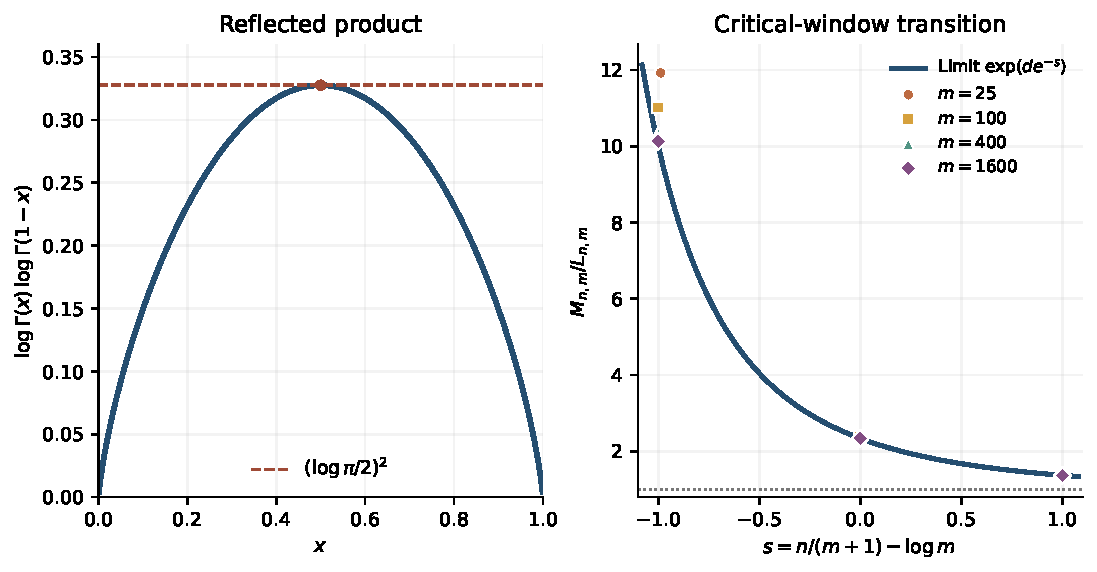
\includegraphics[width=\textwidth]{figures/gamma_joint.pdf}
\caption{Left: the reflected product and its sharp maximum. Right: the
critical-window profile $\exp(d e^{-s})$ with numerical quadrature
for $m=25,100,400,1600$. The horizontal dotted line is the fixed-$m$
leading reference ratio one. The analytic theorem proves the profile;
the plotted points are numerical diagnostics.}
\label{cont26:fig:gamma-joint}
\end{figure}
